\section{Training an \ac{RNN} for \ac{ASR}}\label{ds}
As stated above, this project does not aim at training a state of the art \ac{STT} engine. Because the \ac{SW} algorithm used for local alignment is tolerant to a certain amount of errors in the transcripts, the \ac{RNN} need only be \textit{good enough} for the task at hand (\ac{FA}). If such a network can be trained under the given circumstances it could be used in the \ac{ASR} stage of the pipeline. The pipeline would then become become self-contained and would not ne dependent on a commercial solution that cannot eb tuned and whose inner workings are unknown. Furthermore such a \ac{RNN} would open up to recognizing languages for which there is not a third-party solution yet, such as Swiss German.

\subsection{Related research}

Hier etwas über Transfer Learning (z.B. wie in https://arxiv.org/pdf/1706.00290.pdf) und warum es nicht eingesetzt wurde (CNN anstatt RNN, Zeitaufwand). Layer Freezen bringt ausserdem offenbar auch nix. \parencite{budget}

\subsection{\textit{DeepSpeech}: A reference model}

A \ac{NN} that had quite an impact on \ac{ASR} was \textit{DeepSpeech} \parencite{deepspeech} which reached recognition rates near-par to human performance, despite using a comparably simpler than traditional speech systems. Because the relation between audio signal and text was learned \ac{E2E} the network was also pretty robust to distortions like background noise or speaker variation. An open source implementation of a DeepSpeech model is available from Mozilla \footnote{\url{https://github.com/mozilla/DeepSpeech}}. Since this implementation uses a \ac{LM}, the quality of the model is measured as the percentage of misspelled or wrong words (called \ac{WER}) or as the edit distance (also called Levenshtein distance or \ac{LER}). A pre-trained model for inference of English transcript can be downloaded, which achieves a \ac{WER} of just 6.5\%, which is close to what a human is able to recognize \parencite{mozillajourney}.

\subsection{Exploiting the \textit{DeepSpeech} model}

A model could be trained by providing training-, validation- and test-data for an arbitrary language (e.g. from the \textit{ReadyLingua} corpus). However, this is not the preferred procedure for this project for various reasons:

\begin{enumerate}
	\item The \textit{DeepSpeech} implementation was designed for \ac{ASR}. In such settings a low \ac{WER} is desirable. But this is not the main focus for this project. As a result, the architecture of the Mozilla implementation might be overly complicated for this project, although it might make sense for pure \ac{ASR} tasks. 
	\item The problem with above point is that more complex models usually require more training data. However, as for any neural network, the limiting factor for training a \ac{RNN} is often the lack of enough high quality training data. This becomes especially important when recordings in a minority language should be aligned. 
	\item The implementation requires an (optional) \ac{LM}, which is tightly integrated with the training process which might not be available for the target languages.
\end{enumerate}

For these reasons, the \ac{RNN} architecture of the \textit{DeepSpeech} model was used as a basis for a simplified version, which should (hopefully) require less training data in order to converge and still produce partial transcriptions that can be locally aligned.

\subsection{A simpler \textit{DeepSpeech} model}

An implementation of the \ac{RNN} used for \ac{STT} in the previous IP8 project was done in Python using Keras\footnote{\url{https://keras.io}}. This model is further referred to as \textit{previous model}. Unfortunately, this model did not perform well, i.e. it was not able to learn how to infer a transcript from a given sequence of feature vectors from a spectrogram.  Furthermore, performance was a big issue, although the \ac{RNN} used a simpler architecture and no computational power was needed to query a \ac{LM}. Training on aligned speech segments from the \textit{LibriSpeech} corpus was not possible within project time because it would have taken approximately two months when using a single ac{GPU}. This duration is at least consistent with the experience made by the Machine Learning team at Mozilla Research, which used a cluster of 16 \acsp{GPU} that required about a week \parencite{mozillajourney} to train a variant \footnote{the variant used \ac{MFCC} as features whereas the original paper proposed raw spectrograms} of the \ac{RNN} originally proposed in \parencite{ctc_paper}.

For this project, the previous model was closer examined to find out what works best and to help the model converge. After some changes to the previous model architecture for this project, a new model was obtained which was able to learn something meaningful, i.e. it started to infer transcripts that -- although still not perfect -- resembled the ground truth. This model is further referred to as \textit{new model}. Summarized, the following changes were made to the previous model architecture to constitute the new model:

\begin{itemize}
	\item \textbf{Optimizer}: The new model uses \ac{SGD} instead of Adam. Adam was used in the previous model because it is the Optimizer used in the Mozilla implementation of \ac{DS}. However, this optimizer did not seem to work for the simplified model.
	\item \textbf{RNN cell type}: While \ac{LSTM} cells were used for the recurrent layer in the previous model, this was changed back to a simple RNN layer without gates as they appear in \ac{GRU} or \ac{LSTM} cells in the new model. This also corresponded to the original \textit{DeepSpeech} model architecture, which did not use sophisticated gated cells in their recurrent layer for computational reasons.
	\item \textbf{number of features}: While the use of \ac{MFCC} as features was examined in the previous model, the number of features was set to $13$, a value which is found often used in acoustic modelling. The Mozilla implementation of \textit{DeepSpeech} however doubled this number to $26$, which is also what is used in the new model. In spite of the increase in the number of features, this value is still much smaller than the $160$ filter banks used in the original \textit{DeepSpeech} model. The amount of training data is therefore still expected to be smaller than in the original model.
\end{itemize}

The final model used in this project was therefore a variant of the original \textit{DeepSpeech} model with the following simplifications:

\begin{itemize}
	\item \textbf{Different application of LM}: In the Mozilla implementation the use of a \ac{LM} is baked in with the training process, i.e. it is integrated in the decoding process. With The edit distance between prediction and ground truth is then included in the loss which is minimized. The simplified model also uses a \ac{LM}, but does not include it in the training process. Instead, the \ac{LM} is applied in some sort of post-processing to improve the quality of the decoded predictions.
	\item \textbf{Different features}: MFCC with 26 filter banks instead of Spectrogram with 161 filterbanks, because that's what the Mozilla implementation uses
	\item No convolution in first layer
	\item LSTM instead of SimpleRNN
	\item \textbf{smaller alphabet}: The Mozilla implementation uses an alphabet of 29 characters (${a,b,c,...,z, space, apostrophe, blank}$), which is also what is proposed in the \textit{DeepSpeech} paper. This is due to the fact that apostrophes are frequently found in English word tokens (like \textit{"don't"} or \textit{"isn't"}). For simplification and also because a model should be trainable for any language, this character was dropped from the alphabet used in this project and also removed from the transcripts of all training samples by the normalization process. It is expected that missing apostrophes can be fixed by post-processing the inferred transcript with a \ac{LM}.
	\item \textbf{no context}: The \textit{DeepSpech} paper proposes using combining each feature vector $x_t$ (a frame in the spectrogram) with $C \in \left\{ 5,7,9 \right\}$ context frames. This context frame was dropped to keep the nuber of features in the input layer small. As a result, the first layer in the model only depends on the $26$ features of the feature vector $x_t$.
	\item \textbf{no convolution in input layer}: The \textit{DeepSpeech} paper proposes a series of optimization to reduce computational cost. Among these optimization is a convolution over time in the input layer with by striding with step size $2$. Because the context frame was dropped in this project, the striding was also not applied in order not to lose the information from the intermediate frames.
\end{itemize}


Figure \ref{model_architecture} shows the architecture proposed in the \textit{DeepSpeech} with the changes applied for this project. It looks similar to the one shown in the paper. Note the missing context frame, the use of \ac{MFCC} features and \ac{LSTM} cells in the recurrent layer.

\begin{figure}
	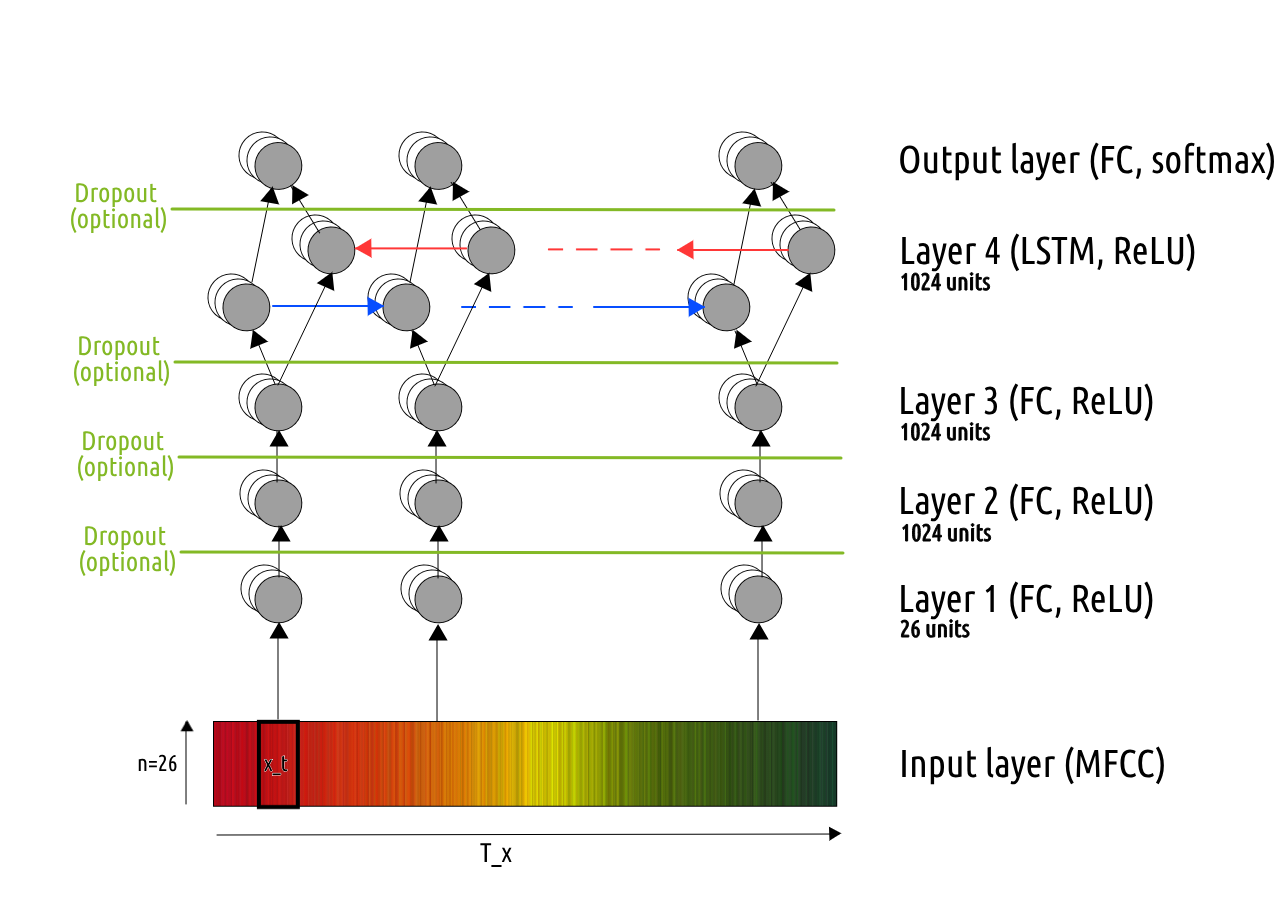
\includegraphics[width=\linewidth]{./img/model_architecture.png}
	\caption{architecture of the simplified model}
	\label{model_architecture}
\end{figure}